سوال ۲

\subsection*{۱.۲}

برای ماشین متناهی غیرقطعی داده شده، ماشین متناهی قطعی‌ای طراحی کردیم که پذیره‌ی همان زبان است صرفا. (رشته‌های عضو زبان را می‌پذیرد و رشته‌های غیرعضو زبان را نمی‌پذیرد.)

در ابتدا استیت‌ها و تابع انتقال DFA مذکور را می‌نویسیم.


فرض می‌کنیم
$L_1$
زبانی می‌باشد که حتما با a شروع می‌شود، تعداد a و b هایش برابر است و اختلاف a و b تا هر جایی حداکثر ۱ است، از اول تا هیچ‌جای دیگری به جز آخر، تعداد a و b برابر نمی‌شود.

همچنین فرض می‌کنیم
$L_2$
زبانی می‌باشد که حتما با b شروع می‌شود، تعداد a و b هایش برابر است و اختلاف a و b تا هر جایی حداکثر ۱ است، از اول تا هیچ‌جای دیگری به جز آخر، تعداد a و b برابر نمی‌شود.

پس داریم:

$$L = (L_1 \cup L_2)^*$$
پس بدست می‌آید که:
$$L_1 = ab , L_2 = ba$$

حالا اگر زبان
$L_3$
را به این شکل تعریف کنیم که زبانی می‌باشد که حتما با a شروع می‌شود، تعداد a و b هایش برابر است و اختلاف a و b تا هر جایی حداکثر ۲ است، از اول تا هیچ‌جای دیگری به جز آخر، تعداد a و b برابر نمی‌شود.

همچنین زبان 
$L_4$
را به این شکل تعریف کنیم که زبانی می‌باشد که حتما با b شروع می‌شود، تعداد a و b هایش برابر است و اختلاف a و b تا هر جایی حداکثر ۲ است، از اول تا هیچ‌جای دیگری به جز آخر، تعداد a و b برابر نمی‌شود.

به طور بازگشتی بدست می‌آوریم که:
$$L_3 = a(ab)^*b$$
$$L_4 = b(ba)^*a$$
پس در نهایت برای تعریف L داریم:
$$L = (a(ab)^*b \cup b(ba)^*a)^*$$

\subsection*{۲.۲}

ماشین قطعی مربوط به هر کدام از زبان‌ها را حالا رسم می‌کنیم.
برای زبان
$L_3$
خواهیم داشت:

\begin{center}
	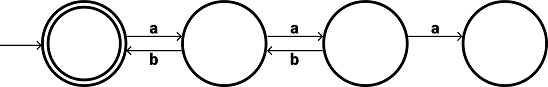
\includegraphics{DFA15}
\end{center}

همچنین برای زبان
$L_4$
خواهیم داشت:

\begin{center}
	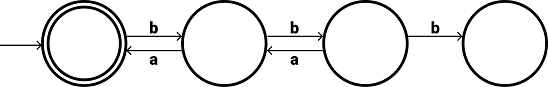
\includegraphics{DFA16}
\end{center}

حالا با ترکیب این دو DFA ، ماشین قطعی برای کل عبارت منظم را بدست می‌آوریم:

\begin{center}
	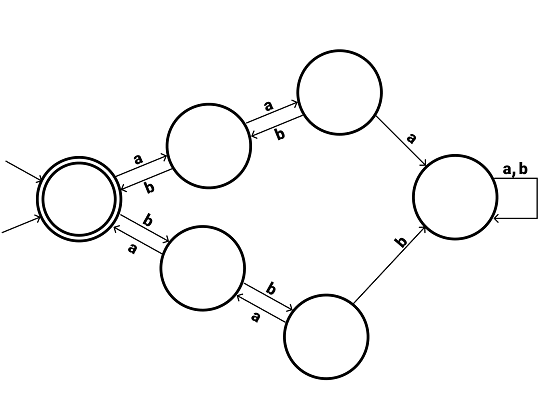
\includegraphics{DFA17}
\end{center}

\subsection*{۳.۲}

برای بدست آوردن ماشین مکمل ماشین موردنظر، حالات accept و reject را جابه‌جا می‌کنیم. در نتیجه مایشن مکمل می‌شود:

\begin{center}
	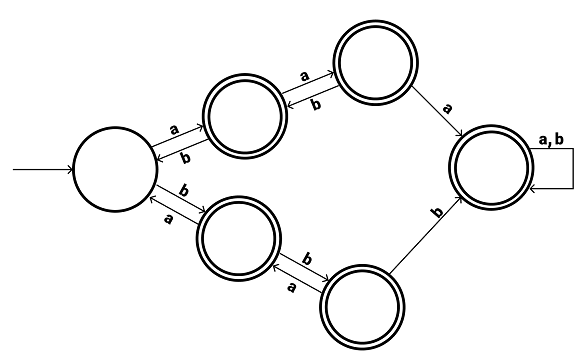
\includegraphics{DFA18}
\end{center}

حالا برای عبارت منظم، اول این DFA را به GNFA تبدیل می‌کنیم. تفاوت این است که این‌جا باید یک استیت accept باید داشته باشیم، در نتیجه استیت‌های accept این DFA را با یک یال اپسیلون به یک استیت جدید وصل می‌کنیم. اسم آن استیت رو accept می‌گذاریم و این NFA بدست می‌آید:

\begin{center}
	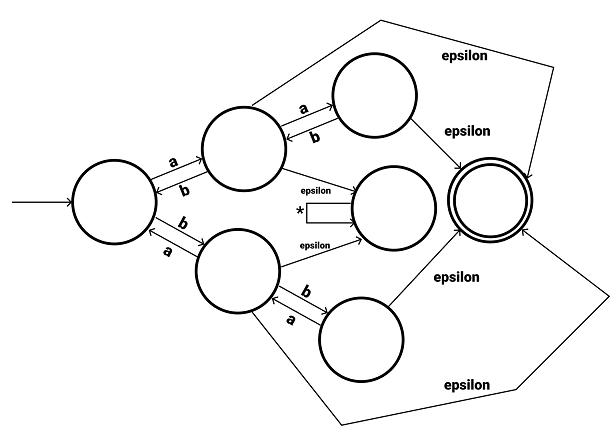
\includegraphics{DFA20}
\end{center}

حالا تبدیل GNFA به عبارت منظم را انجام می‌دهیم:

\begin{center}
	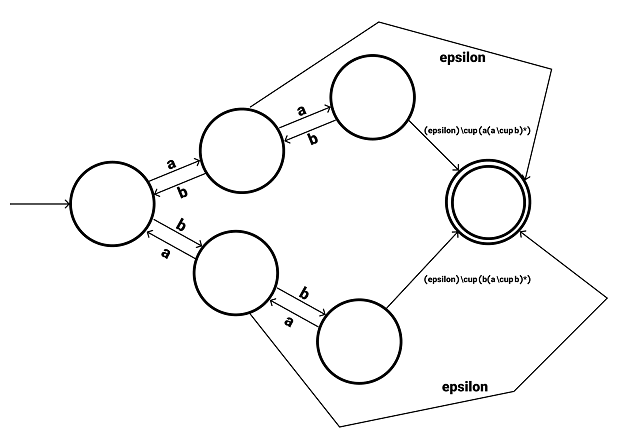
\includegraphics{DFA19}
\end{center}

حالا ۲ راس پایینی را حذف می‌کنیم.

\begin{center}
	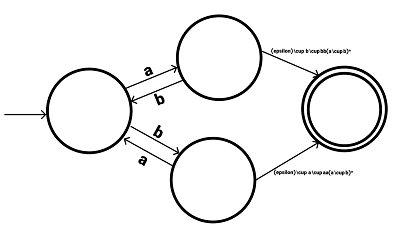
\includegraphics{DFA21}
\end{center}

همچنین ۲ راس دیگر را نیز حذف می‌کنیم.

\begin{center}
	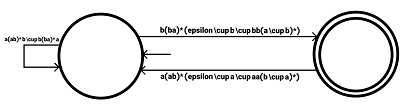
\includegraphics{DFA22}
\end{center}

و در نهایت داریم:

\begin{center}
	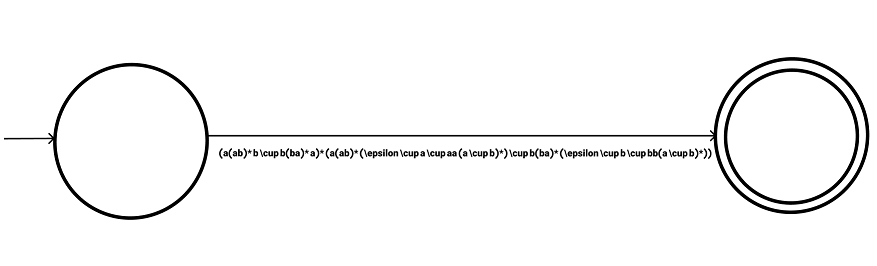
\includegraphics{DFA23}
\end{center}

پس در نهایت به DFA ای می‌رسیم با یالِ
$$
(a(ab)^* b \cup b(ba)^* a)^* (a(ab)^* (\epsilon \cup a \cup aa (a \cup b)^*) \cup b(ba)^* (\epsilon \cup b \cup bb(a \cup b)^*))
$$